\documentclass[a4paper]{article}
\usepackage[spanish,es-lcroman]{babel}
\usepackage[utf8]{inputenc}
\spanishdecimal{.}
\usepackage{bm}
\usepackage{amssymb}
\usepackage{mathtools}
\usepackage{amsmath}
\usepackage{geometry}
\usepackage{parskip}
\usepackage{graphicx}
\usepackage{listings}
\usepackage{xcolor}
\usepackage{float}
\usepackage{tikz}
\usepackage{multicol}
\usepackage{enumitem}
\usepackage{subcaption}
\usepackage{animate}
\definecolor{mygreen}{rgb}{0,0.6,0}
\definecolor{mypurple}{rgb}{0.7,0.3,0.7}
\lstset{
	language=Python,
	backgroundcolor=\color{white},
	frame=none,
	%
	basicstyle=\tt,
	commentstyle=\itshape\color{mygreen},
	keywordstyle=\color{magenta},
	identifierstyle=\color{cyan},
	stringstyle=\color{mypurple},
	showstringspaces=false,
	%
	numbers=none,
	%	numberstyle=\color{gray},
	firstnumber = 1,
	stepnumber=2,
	tabsize =2,
	%
	columns=flexible,
	breaklines=true
}
\lstset{
     literate=%
         {á}{{\'a}}1
         {í}{{\'i}}1
         {é}{{\'e}}1
         {ý}{{\'y}}1
         {ú}{{\'u}}1
         {ó}{{\'o}}1
         {ě}{{\v{e}}}1
         {š}{{\v{s}}}1
         {č}{{\v{c}}}1
         {ř}{{\v{r}}}1
         {ž}{{\v{z}}}1
         {ď}{{\v{d}}}1
         {ť}{{\v{t}}}1
         {ň}{{\v{n}}}1
         {ů}{{\r{u}}}1
         {Á}{{\'A}}1
         {Í}{{\'I}}1
         {É}{{\'E}}1
         {Ý}{{\'Y}}1
         {Ú}{{\'U}}1
         {Ó}{{\'O}}1
         {Ě}{{\v{E}}}1
         {Š}{{\v{S}}}1
         {Č}{{\v{C}}}1
         {Ř}{{\v{R}}}1
         {Ž}{{\v{Z}}}1
         {Ď}{{\v{D}}}1
         {Ť}{{\v{T}}}1
         {Ň}{{\v{N}}}1
         {Ů}{{\r{U}}}1      
         {s̄}{{\={s}}}1
         {ñ̄}{{\~{n}}}1
         {Ñ}{{\~{Ñ}}}1
}

\newenvironment{sidefig}[1]
{\noindent\begin{minipage}[c]{#1\textwidth}}
	{\vfill\end{minipage}}
\newcommand{\herefig}[1]{%
\end{minipage}
\hfill
\noindent\begin{minipage}[c]{#1\textwidth} 
	\centering\vfill
}

\author{Celia Rubio Madrigal}
\title{Práctica 6 - GCOMP}
\date{3 de mayo de 2022}

\begin{document}
	\maketitle
	
	\tableofcontents
	
	\vfill
	
	\begin{center}
		\animategraphics[method=ocg,width=0.45\paperwidth,loop,autoplay]{6}{img/3_}{1}{20}\renewcommand{\thefootnote}{}\footnote{$^*$Para ver este gráfico en movimiento, se recomienda abrir este PDF en Adobe Reader u Okular.}
	\end{center}
	
	
	\vfill
	\newpage
	
	\section{Introducción}
	En esta práctica calcularemos, analizaremos y trazaremos sobre una gráfica la discretización de un sistema dinámico continuo. El sistema que vamos a tratar es el oscilador con dos mínimos, que forma parte de la familia de los osciladores. Son unas ecuaciones muy relevantes y útiles para el mundo de la física, usadas, por ejemplo, en sistemas de muelles, en electrónica, o en cuántica, entre otros campos.
	
	El sistema describe la evolución de la posición y el momento con respecto al tiempo; se trata, por tanto, de una variedad simpléctica con coordenadas $(q(t),p(t))\in\mathbb{R}^2$. El hamiltoniano de nuestro sistema es: $ H(q,p) = p^2 + \frac{1}{4} (q^2-1)^2 $. Y se puede deducir que el sistema cumple estas dos ecuaciones: $ \ddot{q} = -2q(q^2-1)$, y $p = \frac{\dot{q}}{2} $.
	
	
	\section{Material usado y metodología}
	Partimos de un conjunto de condiciones iniciales $D_0=[0,1]\times[0,1]$, que discretizaremos de distintas maneras para cada apartado. Además, discretizaremos el parámetro temporal $t = n\delta\in[0,\infty)$, donde $n\in\mathbb{N}_0$ y $\delta$ también dependerá para cada apartado.
	
	Discretizamos las derivadas de $q$ mediante diferencias finitas. Llamando $q_k \coloneqq q(k\delta)$, tenemos expresado $q_{n+2}$ a partir de $q_{n+1}$ y $q_n$, solo teniéndolo que despejar de la siguiente ecuación:
	
%	\[ 2p(t) = \dot{q}(t) = 
%	\lim_{h\to 0} \frac{q(t+h)-q(t)}{h} \approx 
%	 \frac{q(t+\delta)-q(t)}{\delta} = 
%	 \frac{q_{n+1}-q_n}{\delta}
%	\]
	
	\[ -2q_n\cdot(q_n^2-1) = \ddot{q}(t) = 
	\lim_{h\to 0} \frac{\dot{q}(t+h)-\dot{q}(t)}{h} \approx 
	\frac{q(t+2\delta)-2q(t+\delta)+q(t)}{\delta^2} =
	\frac{q_{n+2}-2q_{n+1}+q_n}{\delta^2}
	\]
	
	\subsection{Apartado \textit{i})}
	En el primer apartado, fijamos $\delta= 10^{-3}$. Hemos escogido 16 valores en $D_0$ como nuestras condiciones iniciales. En concreto, una malla equidistante de 4 por 4 en las variables $q$ y $p$. Consideramos sus órbitas en el sistema.  
	
	Llamando al método \verb+simplectica+, se calcula la órbita de cada punto inicial hasta el paso $n = \frac{20}{\delta}$ (ya que no podemos calcular sus valores hasta el infinito) y se dibuja en una gráfica. De esta manera, estamos representando una discretización del espacio fásico $D_{(0,\infty)}$.
	
	
	\subsection{Apartado \textit{ii})}
	En el segundo apartado, calculamos el valor del área $D_t$ que ocupan los puntos iniciales, que comenzaron en $D_0$, en el instante $t=0.25$. Ahora vamos a tomar 10 puntos por variable, luego tendremos 100 puntos en total.
	
	El teorema de Liouville enuncia que el área de $D_t$ es invariante con respecto a la variable temporal. Como el área de $D_0$ es 1 (es el cuadrado unidad), el valor que calculemos tendrá que ser también 1, con un posible margen de error.
	
	Para calcular el área, tomaremos el área de la envoltura convexa de los puntos. Le restaremos las dos áreas de las envolturas convexas de las aristas superior y derecha, que se curvan y hacen que la figura no sea convexa.
	
	Además, calcularemos el error que estamos cometiendo al tomar la aproximación discreta, mediante el ajuste de $\delta\in[10^{-4},10^{-3}]$, de cuyo intervalo tomaremos 10 valores equidistantes para comparar sus áreas resultantes entre sí.
	
	\subsection{Apartado \textit{iii})}
	En el tercer apartado, fijaremos de nuevo $\delta=10^{-3}$. De nuevo, dibujaremos los puntos del sistema para distintos tiempos. Tomaremos una malla equidistante de 20 por 20 en $D_0$ como condiciones iniciales.
	
	Esta vez los instantes $t$ serán equidistantes en el intervalo $[0,5]$. Con las 20 gráficas que resulten, realizaremos una animación.
	
	\section{Resultados y conclusiones}
	
	\subsection{Apartado \textit{i})}
	En la figura \ref{fig:1} se muestra la gráfica de las 16 órbitas finales de nuestro sistema. Se puede observar que parece tener dos mínimos, como bien indica su nombre.
	
	
	\subsection{Apartado \textit{ii})}
	En la figura \ref{fig:2} se muestra la gráfica de los 100 puntos del sistema, que comenzaron como una malla en el cuadrado unidad, en el instante $t=0.25$ y con $\delta=10^{-3}$. Los puntos verdes y naranjas forman las dos áreas convexas de los laterales que se han restado al valor del área total. 
	
	El valor del área para este $\delta$ es de $0.9999 \pm 0.0001$. Para $\delta=10^{-4}$, es de $0.9997 \pm 0.0001$, y entre medias los valores decrecen al decrecer $\delta$. Tomaremos, por tanto, el área total como $0.9998 \pm 0.0002$, con el valor siendo la media entre ambos valores extremos, y el error su resta. El resultado es muy cercano al valor de 1 que esperábamos, así que hemos verificado que el teorema de Liouville se cumple.
	
	\begin{multicols}{2}
		\begin{figure}[H]
			\centering
			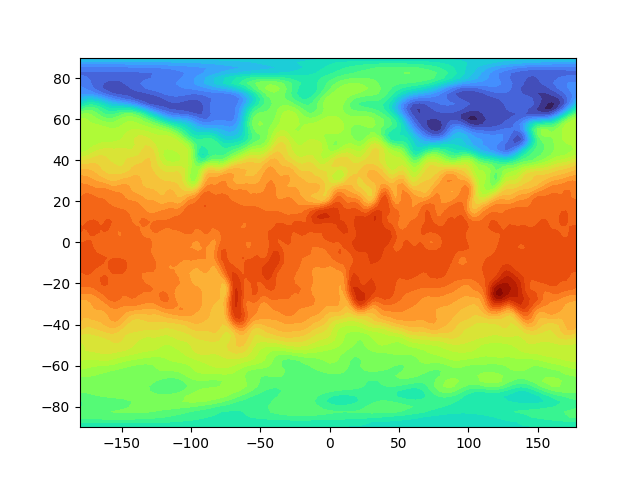
\includegraphics[width=0.95\linewidth]{1}
			\caption{Espacio fásico del sistema.}\label{fig:1}
		\end{figure}
		
		\begin{figure}[H]
			\centering
			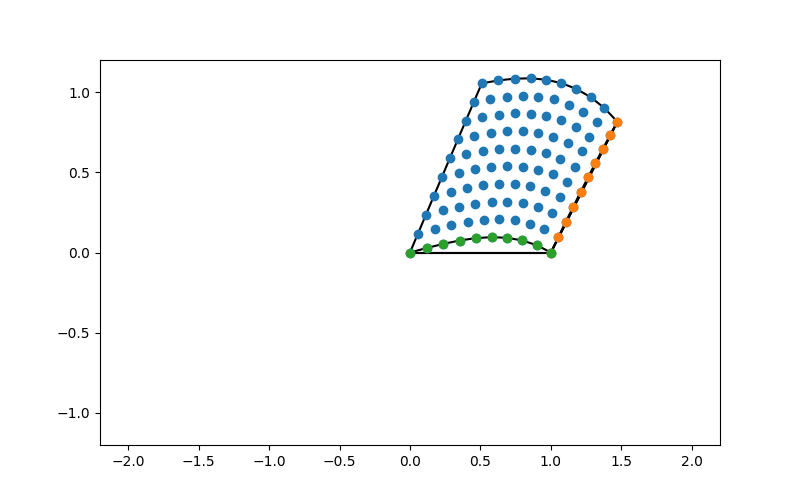
\includegraphics[width=0.95\linewidth]{figs/2-0.001000.png}
			\caption{$D_{0.25}\ (\delta = 10^{-3})$.}\label{fig:2}
		\end{figure}
	\end{multicols}
	
	
	\subsection{Apartado \textit{iii})}
	En los archivos adjuntos, así como en la portada de este trabajo, se encuentra la animación de la sucesión de gráficas de $D_t$ representadas a lo largo de $t\in[0,5]$.
	
	Gracias a estos cálculos y estas representaciones visuales del espacio de fases, comprendemos mejor cómo se comporta este sistema físico. Con nuestros datos podríamos modelar, comparar y predecir un sistema del mundo real con amplias aplicaciones. Por otro lado, hemos comprobado que se cumple el teorema de Liouville para este sistema simpléctico.
	
	\newpage
	\section{Código}\label{codigo}
	
	\lstinputlisting[language=Python]{p6_rubiomadrigalcelia.py}
	
\end{document}
